\question{Câu 7}

Cho một tín hiệu cần xử lý dưới dạng dòng điện, có tầm thay đổi từ $1\,\textsf{mA} - 10\,\textsf{mA}$.

\answer{a}{Thiết kế mạch cho ngõ ra tầm $\mathbf{100}\,\text{mV} - \mathbf{1}\,\textsf{V}$.}

\begin{minipage}{.5\linewidth}
	\begin{figure}[H]
		\centering
		
\includegraphics[width=\linewidth]{./my-chapters/my-images/Question7/debai.png}
	\end{figure}
\end{minipage}
\begin{minipage}{.5\linewidth}
	Thiết lập phương trình quan hệ giữa ngõ vào và ngõ ra:
	\[V_{out} = 100I_{in}\]
\end{minipage}

Để thiết kế mạch $I-V Converter$, nhóm em sử dụng dụng dạng mạch \textbf{Transimpedance Amplifier} như sau:

\begin{figure}[H]
	\centering
	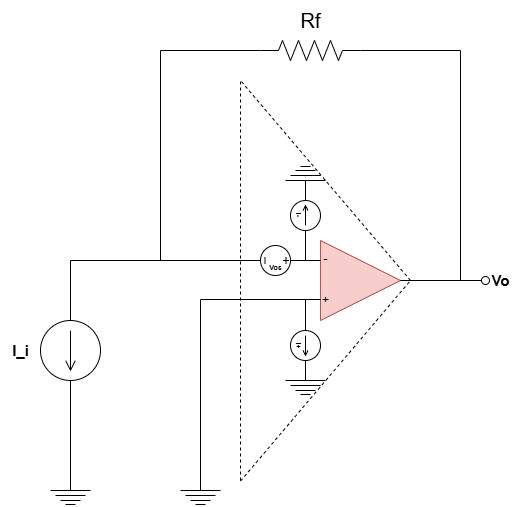
\includegraphics[width=.8\linewidth]{./my-chapters/my-diagrams/Question7/a_non_ideal_module_q7.png}
	\caption{Transimpedance Amplifier Design.}
\end{figure}

Ta xét:

\begin{itemize}[label=-]
	\item Xét $V_{in}$, $V_{os} = 0$, $I_{+} = 0$, $I_{-} = 0$:
	\[ V_{out} = R_{F}I_{in} \]
	
	Với $\Delta I_{in} = 10 - 1 = 9 \,\textsf{mA}$ và $\Delta V_{out} = 1 - 0.1 = 0.9\,\textsf{V}$
	\[ \Rightarrow R_{F} = \dfrac{\Delta V_{out}}{\Delta I_{in}} = \dfrac{0.9}{9\,\textsf{m}} = 100\,\Omega\]
	\item Xét $V_{os}$, $V_{in} = 0$, $I_{+} = 0$, $I_{-} = 0$:
	\[ V_{out} = -V_{os} \]
	\item Xét $I_{+}$ và $I_{-}$, $V_{in} = 0$, $V_{os} = 0$:
	\[ V_{out} = I_{-}R_{F} \]
\end{itemize}

$\Rightarrow$ \finalresult{V_{out} = R_{F}I_{in} \mp V_{os} \pm I_{-}R_{F}}.

\answer{b}{Lựa chọn OPAMP và các linh kiện cần thiết để mạch hoạt động. Lưu ý: \textit{xử lý các thông số không lý tưởng của OPAMP.}}

Ta xét,

\begin{itemize}[label=-]
	\item \textbf{Chọn hệ số khuếch đại của mạch (Gain):} Để có $V_{out} = 100\times I_{in} \Rightarrow R_{F} = 100\,\Omega$
	\item \textbf{Output swing và supply rails:} Với ngõ ra rơi vào tầm $0.1-1\,\textsf{V}$ thì chọn nguồn từ $0\rightarrow 5\,\textsf{V}$ hoặc $\pm5\,\textsf{V}$ trở đi là được.
	\item \textbf{Input offset và Noise:} $\Delta V = - V_{os} + I_{-}R_{F}$
	\begin{itemize}[label=+]
		\item $V_{os}$ phải đủ nhỏ rơi vào tầm $\mu\,\textsf{V}$ để $V_{out} \approx \mu\textsf{V}$, hoặc có thể chọn những con rơi vào tầm \textsf{mV} để sau số không đáng kể.
		\item $I_{-} = \left\{ \begin{matrix}
			\dfrac{1}{2}I_{os} - I_{ib} \\[4pt]
			\dfrac{1}{2}I_{os} + I_{ib}
		\end{matrix} \right.$ thì phải chọn $|I_{os}|$ và $|I_{ib}|$ rơi vào tầm để khi $I_{-}R_{f} = 100I_{-}$ có thể bù trừ với $V_{os}$ được.
	\end{itemize}
\end{itemize}

Từ đó, nhóm em chọn OPAMP: \href{https://www.ti.com/lit/ds/symlink/op07.pdf?ts=1761807672016&ref_url=https%253A%252F%252Fwww.mouser.fr%252F}{\textbf{OP07CD}}.

\begin{figure}[H]
	\centering
%	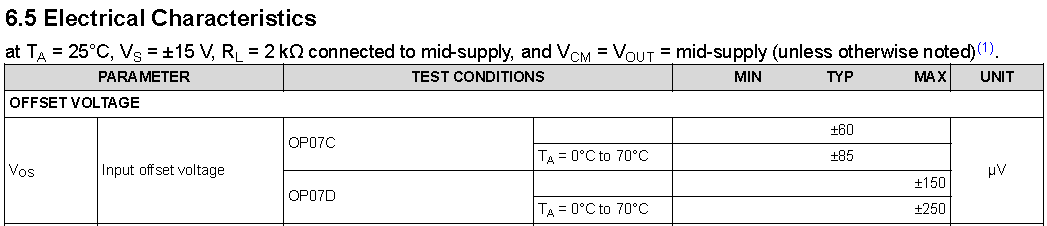
\includegraphics[width=.9\linewidth]{./my-chapters/my-diagrams/Question7/V_os_op07.pdf}
%		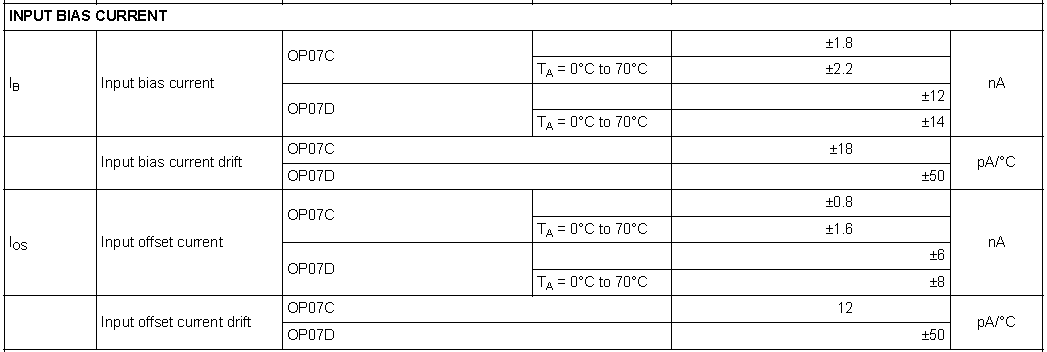
\includegraphics[width=.9\linewidth]{./my-chapters/my-diagrams/Question7/I_bias_current_op07.pdf}
	
\includegraphics[width=.9\linewidth]{./my-chapters/my-images/Question7/datasheet.png}
	\caption{Electrical Characteristics for OP07CD.}
\end{figure}

\begin{itemize}[label=-]
	\item Ta có: $V_{os} = 85\,\mu\textsf{V} \Rightarrow V_{os} = -85\,\mu\textsf{V}$.
	
	\item Ta có: $I_{os} = 1.8\,\textsf{nA}$ và $I_{ib} = 2.2\,\textsf{nA}$
	$\Rightarrow I_{-} = \left\{ \begin{matrix}
		\dfrac{1}{2}I_{os} - I_{ib} = -1.3\,\textsf{nA} \\[4pt]
		\dfrac{1}{2}I_{os} + I_{ib} =  3.1\,\textsf{nA}
	\end{matrix} \right.$ 
	
	$\Rightarrow I_{-}R_{F} = \left[ -0.13, 0.13\right]\,\mu \textsf{V}$
\end{itemize}

$\Rightarrow$ \finalresult{V_{out} = 100I_{in} + \left[ -0.08513\,\textsf{mV}, -0.08487\,\textsf{mV}\right]}.

\answer{c}{Mô phỏng mạch dùng Multisim (hoặc các chương trình tương tự).}

\begin{figure}[H]
	\centering
	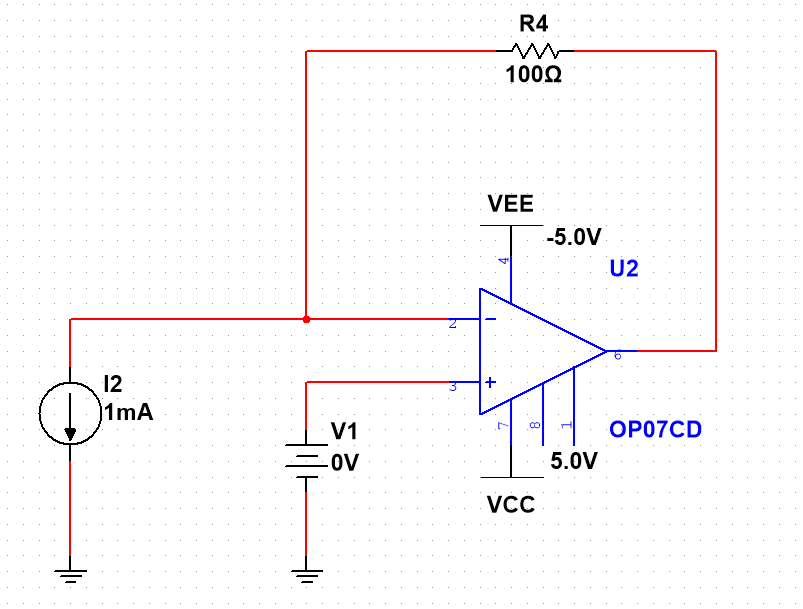
\includegraphics[width=0.7\linewidth]{my-chapters/my-images/Question7/a_mach_thietke.png}
	\caption{Sơ đồ mạch của mạch Transimpedance Amplifier.}
\end{figure}

Tiến hành DC sweep để đo điện áp ngõ ra khi điện áp ngõ vào thay đổi từ $1\,\textsf{mA} \rightarrow 10\,\textsf{mA}$,

\begin{figure}[H]
	\centering
	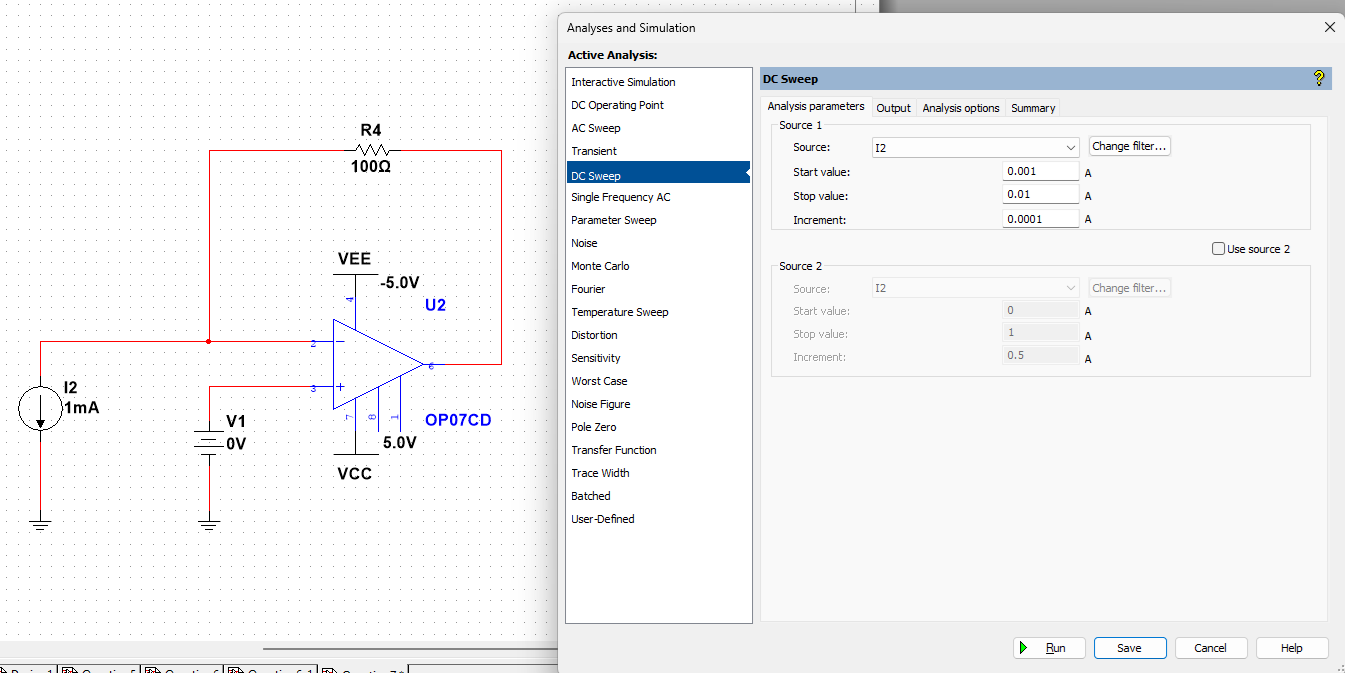
\includegraphics[width=0.7\linewidth]{my-chapters/my-images/Question7/a_dcSeep.png}
	\caption{Tiến hành chạy DC sweep.}
\end{figure}

Kết quả,

\begin{figure}[H]
	\centering
	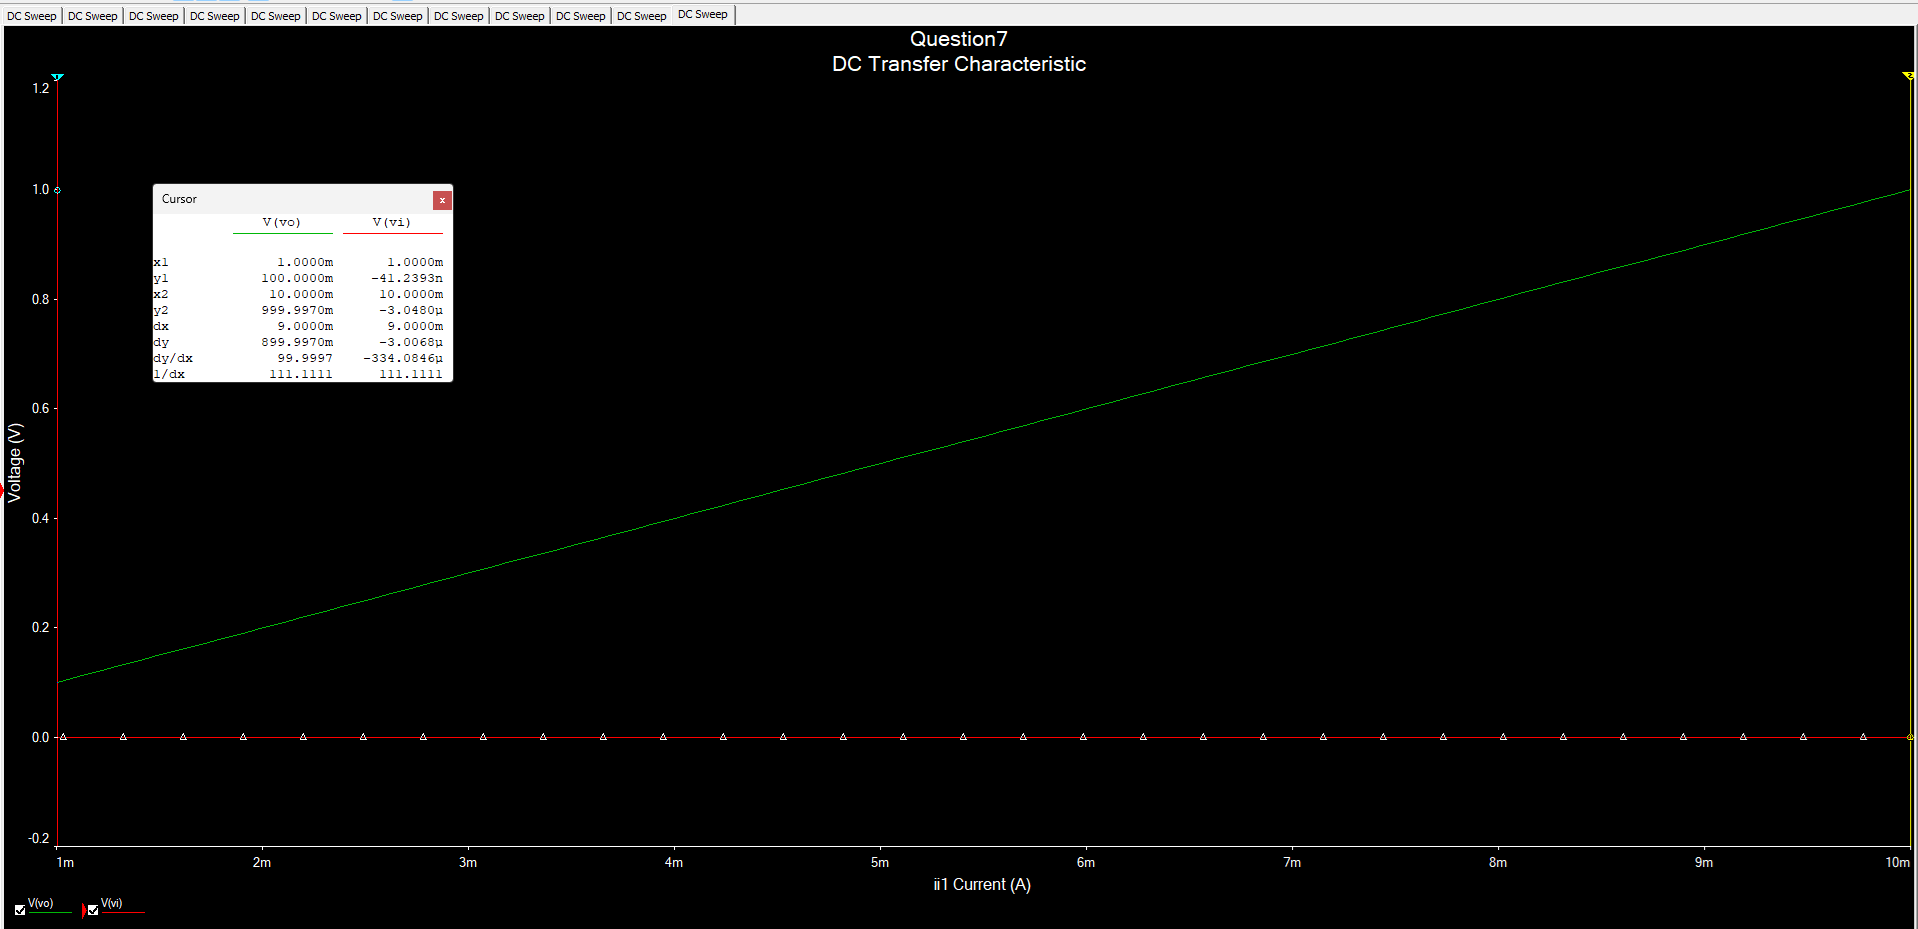
\includegraphics[width=\linewidth]{my-chapters/my-images/Question7/b_dcsweep_hinh.png}
	\caption{Kết quả của ngõ ra sau khi chạy DC sweep.}
\end{figure}

Kiểm tra sai số,

\begin{minipage}{.5\linewidth}
	\begin{figure}[H]
		\centering
		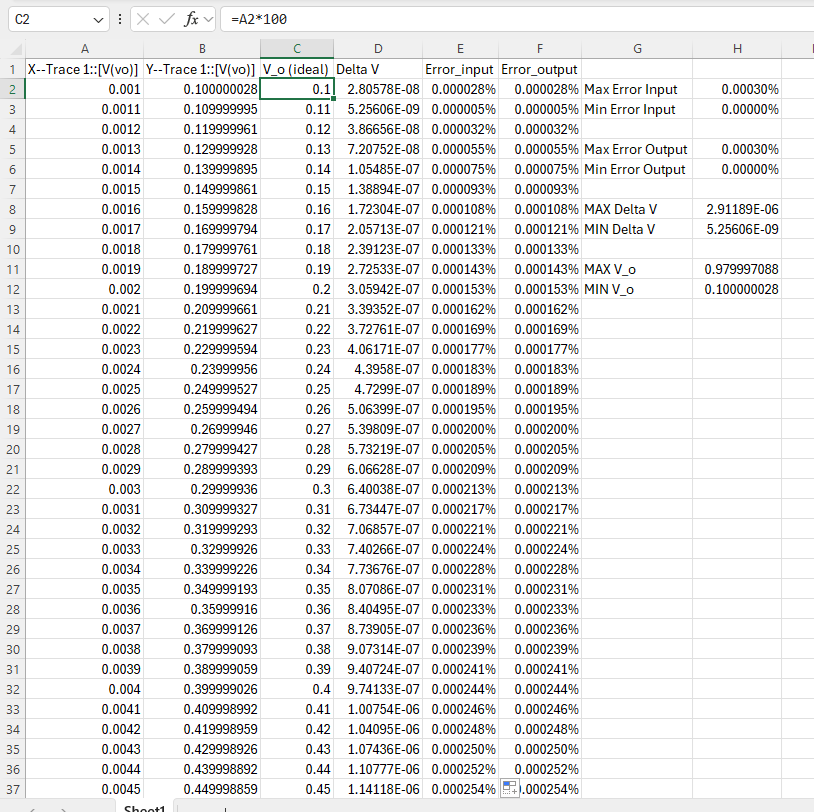
\includegraphics[width=\linewidth]{./my-chapters/my-images/Question7/saiso.png}
	\end{figure}
\end{minipage}
\begin{minipage}{.5\linewidth}
	\begin{itemize}[label=-]
		\item Giá trị $V_{ideal}$ được tính bằng cách lấy $I_{in}\times 100$
		\item Giá trị $\Delta V = | V_{o} - V_{ideal} |$
		\item Giá trị \finalresult{\Delta V _{max} =2.91189\,\mu\textsf{V}} và \finalresult{\Delta V _{min} = 5.25606\,\textsf{nV}}
		\item Sai số ở ngõ ra rơi vào tầm \finalresult{\Delta V_{o_{max}} = 0.00030\%} và \finalresult{\Delta V_{o_{min}} = 0.00000\%}
	\end{itemize}
\end{minipage}